\documentclass[tikz,border=10mm]{standalone}
\usepackage{tikz}
\usetikzlibrary{arrows.meta, positioning, fit, calc}

\begin{document}
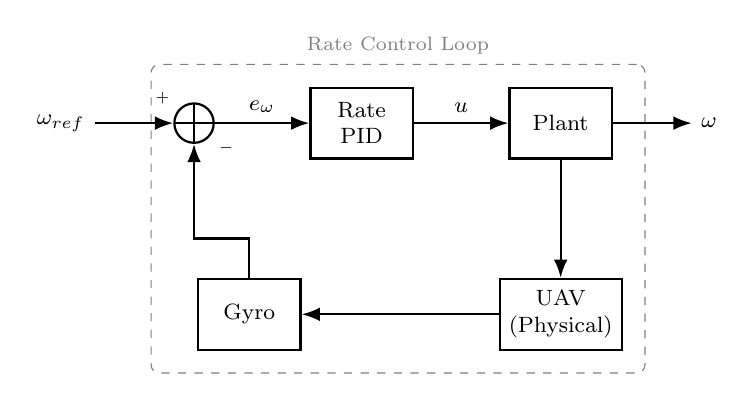
\begin{tikzpicture}[
    node distance = 1.0cm and 1.2cm,
    >=Latex,
    font=\footnotesize,
    block/.style = {draw, rectangle, minimum height=0.9cm, minimum width=1.3cm, align=center, thick},
    sum/.style = {draw, circle, minimum size=0.5cm, thick, path picture={\draw (path picture bounding box.north) -- (path picture bounding box.south) (path picture bounding box.west) -- (path picture bounding box.east);}},
    group/.style = {draw, dashed, inner sep=8pt, gray, rounded corners=3pt},
    arrow/.style = {->, thick}
]

% =========================================================
% KEY DIFFERENCE FOR RATE MODE: 
% Input is Rate Setpoint (Omega_ref) directly to the Rate Loop
% =========================================================

% Input
\node (omega_ref) {$\omega_{ref}$};

% Rate Loop Summing Junction (S2 in previous diagram)
\node[sum, right=1.0cm of omega_ref] (sum) {};

% PID Controller
\node[block, right=1.2cm of sum] (pid) {Rate\\PID};

% Plant
\node[block, right=1.2cm of pid] (plant) {Plant};

% Output
\node[right=1.0cm of plant] (omega) {$\omega$};

% =========================================================
% FEEDBACK PATH PHYSICAL COMPONENTS
% =========================================================
\node[block, below=1.5cm of plant] (uav) {UAV\\(Physical)};
\node[block, left=2.5cm of uav] (gyro) {Gyro};

% =========================================================
% WIRING: FORWARD PATH
% =========================================================
\draw[arrow] (omega_ref) -- (sum);
\draw[arrow] (sum) -- node[above]{$e_\omega$} (pid);
\draw[arrow] (pid) -- node[above]{$u$} (plant);
\draw[arrow] (plant) -- (omega);

% Signs for Summing Junction
\node[above left=-2pt and 0pt of sum] {\tiny +};
\node[below right=-2pt and 0pt of sum] {\tiny $-$};

% =========================================================
% WIRING: FEEDBACK PATH
% =========================================================
% Plant to UAV
\draw[arrow] (plant.south) -- (uav.north);

% UAV to Gyro
\draw[arrow] (uav.west) -- (gyro.east);

% Gyro to Summing Junction
% Route: Up from Gyro, then Left to Sum
\draw[arrow] (gyro.north) -- ++(0, 0.5) -| (sum.south);

% =========================================================
% GROUPS (dashed boxes)
% =========================================================
\node[group, fit=(sum)(pid)(plant)(uav)(gyro), label={[gray, font=\scriptsize]above:Rate Control Loop}] {};

\end{tikzpicture}
\end{document}
